\chapter{Final Model Architecture}\label{ch:architecture}

This chapter explains the final system saved and used by the application. The
installed model is a one-lead MLII beat classifier. It does not use two ECG
leads, does not retrain during live use, and does not make an arrhythmia
decision directly from the autoencoder threshold. The final decision is made by
two supervised Extra Trees models. Both receive the same 242-value feature
vector.

\section{Architecture in one sentence}

For each detected MLII heartbeat, the system takes a 512-sample window aligned
to the R peak, builds waveform, rhythm, and normal-reconstruction features,
sends those features to a binary abnormality gate, and sends only gated
abnormal beats to a five-class subtype classifier.

\begin{figure}[H]
\centering
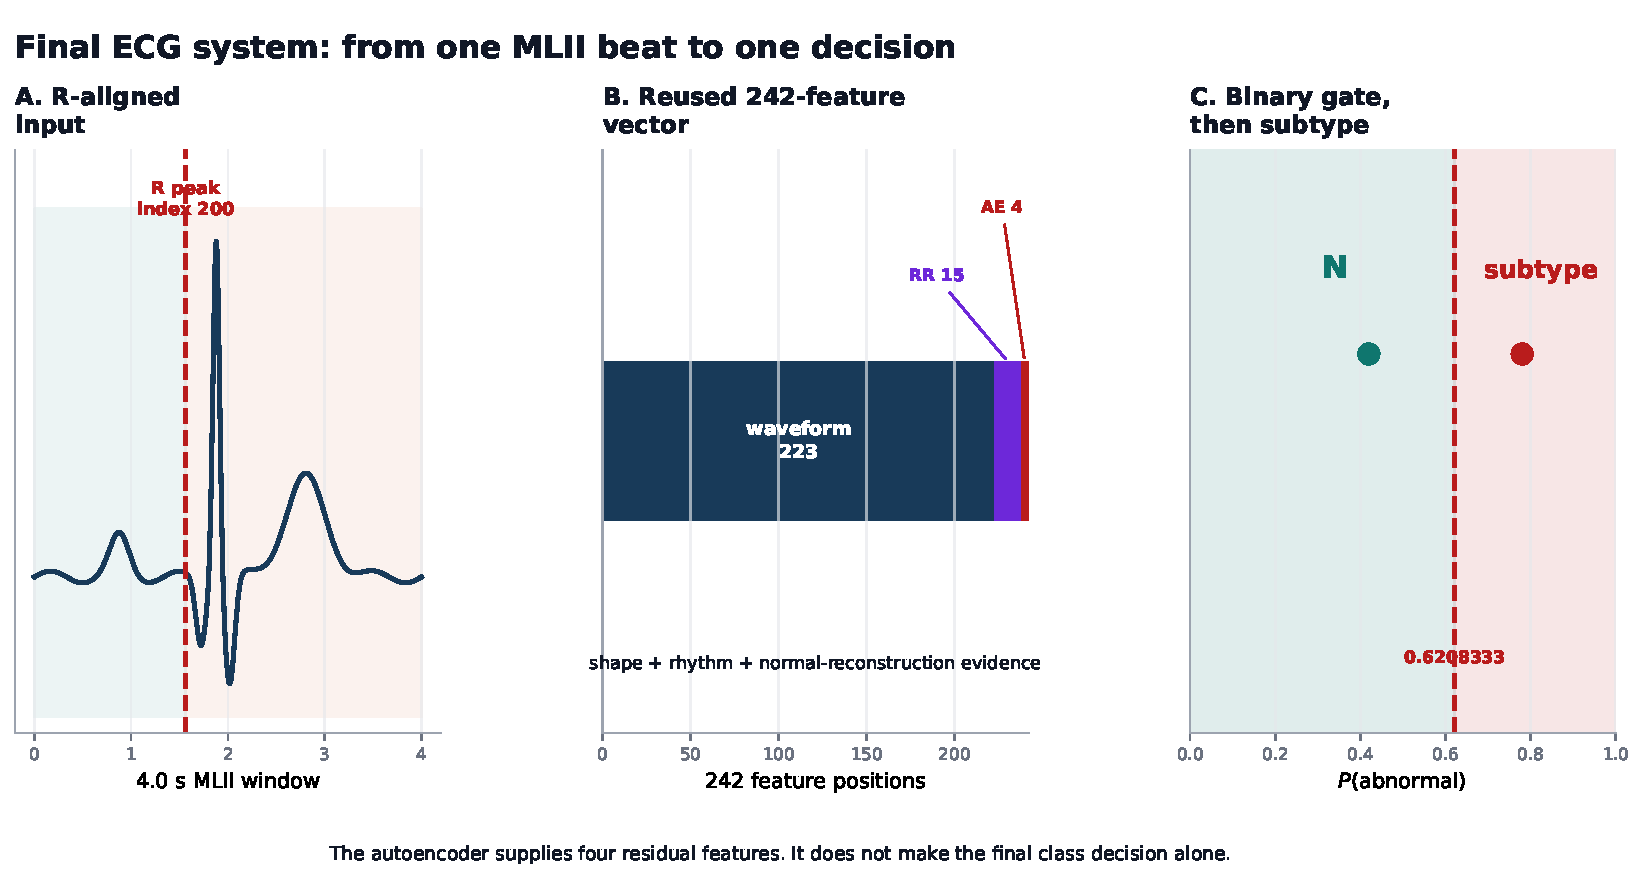
\includegraphics[width=.98\textwidth]{pic/generated/architecture_current_system_flow.pdf}
\caption{Exact runtime order of the final ECG system. The autoencoder supplies
features; the supervised tree models make the final class decision.}
\label{fig:architecture-current-flow}
\end{figure}

\section{Input signal and beat window}

The deployed system accepts one ECG channel. For database replay and final
testing that channel is MIT--BIH MLII, selected by signal name. Records 102 and
104 are excluded because they do not contain MLII. For sensor sessions, the API
requires the user to declare \texttt{lead\_name='MLII'} and rejects other
declared leads. This rule prevents the model from silently scoring a lead that
does not match the supervised training signal.

The classifier is beat based, not arbitrary-window based. The live backend
collects MLII samples, detects R peaks, and waits until enough rhythm context
is available. For a scorable beat, it extracts a fixed 512-sample window at
128 Hz:
\begin{itemize}
\item 200 samples before the R peak;
\item 312 samples after the R peak;
\item total duration of 4.0 seconds.
\end{itemize}
This same window geometry is used in the final temporal-holdout experiment and
in the installed session pipeline.

\begin{figure}[H]
\centering
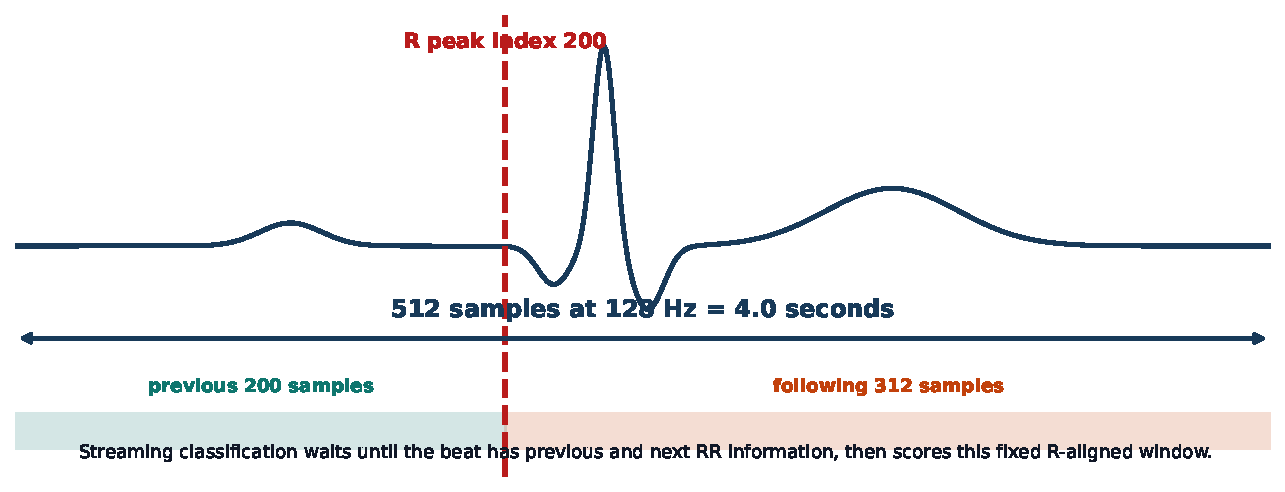
\includegraphics[width=.92\textwidth]{pic/generated/architecture_streaming_window.pdf}
\caption{R-peak-aligned beat window used by the final model. The R peak is at
sample index 200, giving the model pre-QRS context and post-QRS recovery
information.}
\label{fig:architecture-streaming-window}
\end{figure}

\section{Three trained components}

The final system uses three trained components, stored as an autoencoder
checkpoint and a separate hierarchy bundle:
\begin{enumerate}
\item a frozen normal-only autoencoder;
\item a binary Extra Trees abnormality detector;
\item a five-class Extra Trees abnormal-subtype classifier.
\end{enumerate}
The autoencoder is trained first and then frozen. The two supervised tree
models are then fitted on MLII features from the temporal development portion
of MIT--BIH Arrhythmia Database records.

\begin{figure}[H]
\centering
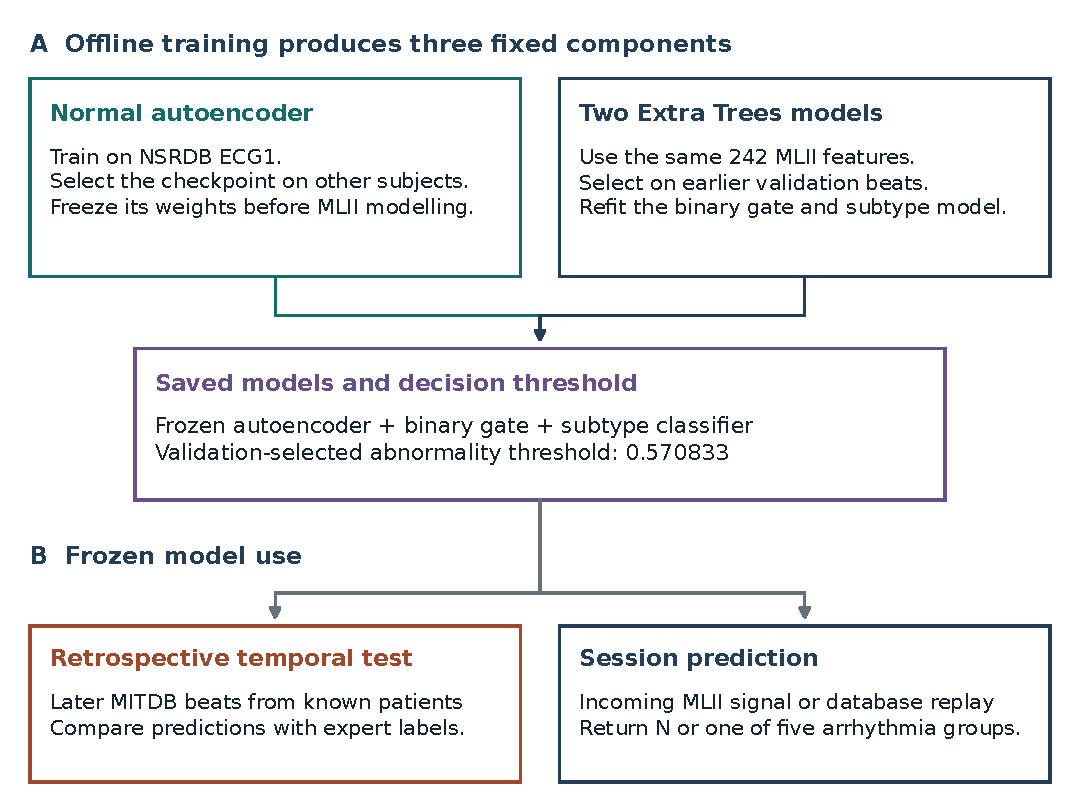
\includegraphics[width=.98\textwidth]{pic/generated/architecture_training_live_map.pdf}
\caption[Training and use of the saved three-component model.]{Training and use
of the saved three-component model. Offline development produces the frozen
autoencoder, binary gate, subtype classifier, and validation-selected threshold.
The same fixed components support retrospective temporal evaluation and session
prediction; session use does not update its parameters.}
\label{fig:architecture-training-live}
\end{figure}

\section{Normal-only autoencoder}

\subsection{Purpose}

The autoencoder is a normal-reconstruction branch. It learns how normal ECG
windows can be reconstructed. The final system then uses reconstruction error
as extra evidence. The autoencoder does not decide ``normal'' or
``arrhythmia'' by itself in the final classifier.

For an input window $x\in\mathbb{R}^{512}$, the autoencoder output is
\begin{equation}
 \widehat x=g_{\phi}(f_{\theta}(x)),
\end{equation}
where $f_{\theta}$ is the encoder and $g_{\phi}$ is the decoder. Training uses
a denoising objective: Gaussian noise with standard deviation 0.03 is added to
the input, but the target remains the clean standardised window. The training
loss is
\begin{equation}
 \mathcal{L}_{AE}=\frac{1}{512}\sum_{t=1}^{512}
 (x_t-\widehat x_t)^2.
 \label{eq:ae-loss-final}
\end{equation}
This objective encourages stable normal morphology instead of copying small
noise patterns \cite{vincent2008denoising}.

\subsection{Network structure}

\begin{figure}[H]
\centering
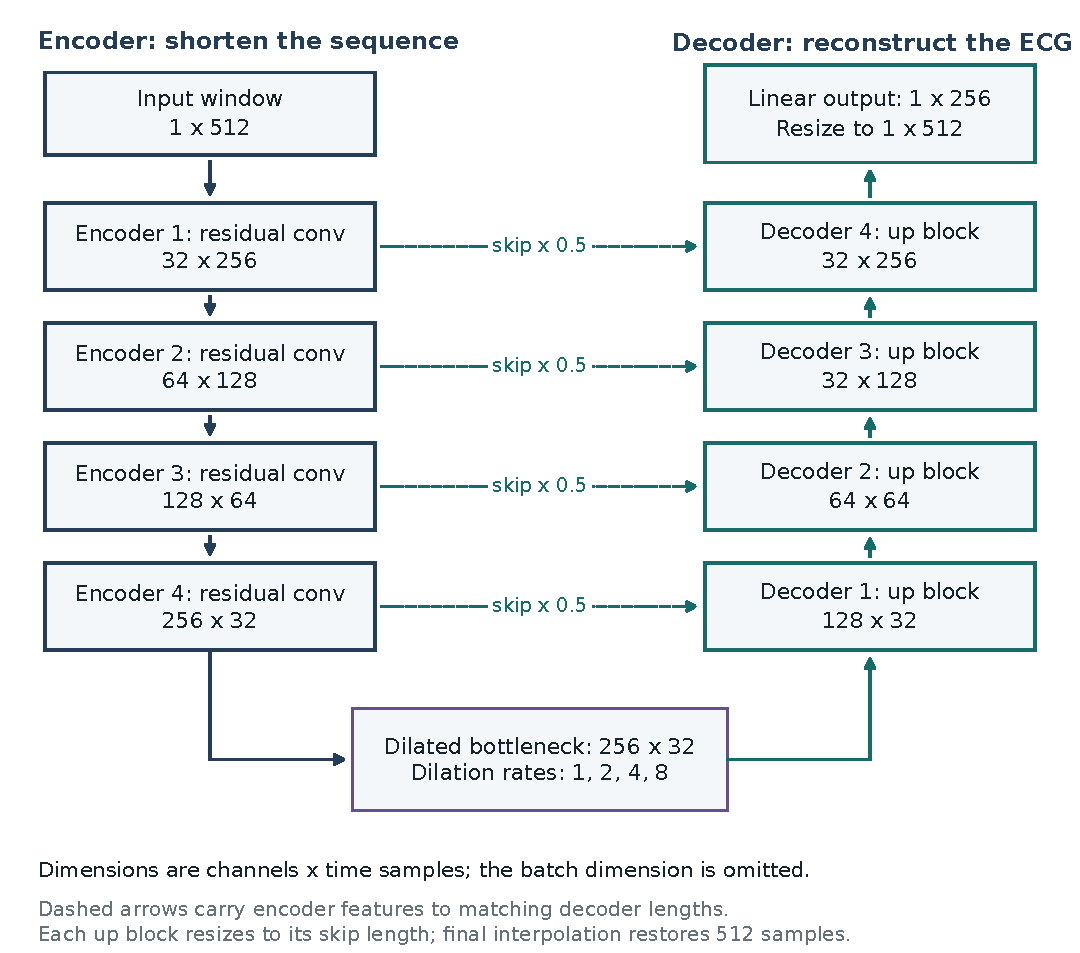
\includegraphics[width=.98\textwidth]{pic/generated/architecture_autoencoder_layers.pdf}
\caption[Autoencoder architecture with verified tensor dimensions.]{Autoencoder
architecture with tensor dimensions verified by a forward pass through the
2,680,641-parameter implementation. Read down the encoder, through the
bottleneck, and up the decoder. Dashed connections concatenate encoder features
scaled by 0.5; decoder outputs match their skip lengths before the final
interpolation restores the 512-sample waveform.}
\label{fig:final-ae-layers}
\end{figure}

Each residual encoder block contains two kernel-seven convolutions, Group
Normalisation, LeakyReLU, dropout, and a residual projection. Four
kernel-three bottleneck blocks use dilation 1, 2, 4, and 8. Dilation increases
the receptive field without deleting time samples. The decoder uses transposed
convolutions and skip connections scaled by 0.5. Each up block resizes its
output to match the corresponding encoder skip. The first up block therefore
returns length 32, the fourth returns length 256, and final linear interpolation
restores length 512. The figure reports these actual tensor dimensions.
The final layer is linear
because the standardised ECG signal contains positive and negative values.

\subsection{Normal-reference data and checkpoint}

The autoencoder checkpoint was developed from complete recordings of all 18
subjects in the MIT--BIH Normal Sinus Rhythm Database. Fifteen subjects supply
288,673 fitting windows and three different subjects supply 57,177 validation
windows. The selected NSRDB header channel is \texttt{ECG1}. The database does
not document this channel as anatomical Lead II, so the report treats it as a
normal ECG reference channel rather than renaming it MLII \cite{nsrdb}.

The final checkpoint uses Adam, learning rate 0.001, batch size 256, and two
epochs. Validation MSE changed from 0.061195 after epoch 1 to the best saved
value, 0.061193, after epoch 2. The autoencoder artifact also stores a
normal-residual threshold of 0.158893, but the final hierarchy does not use
that threshold as the final arrhythmia rule.

\begin{figure}[H]
\centering
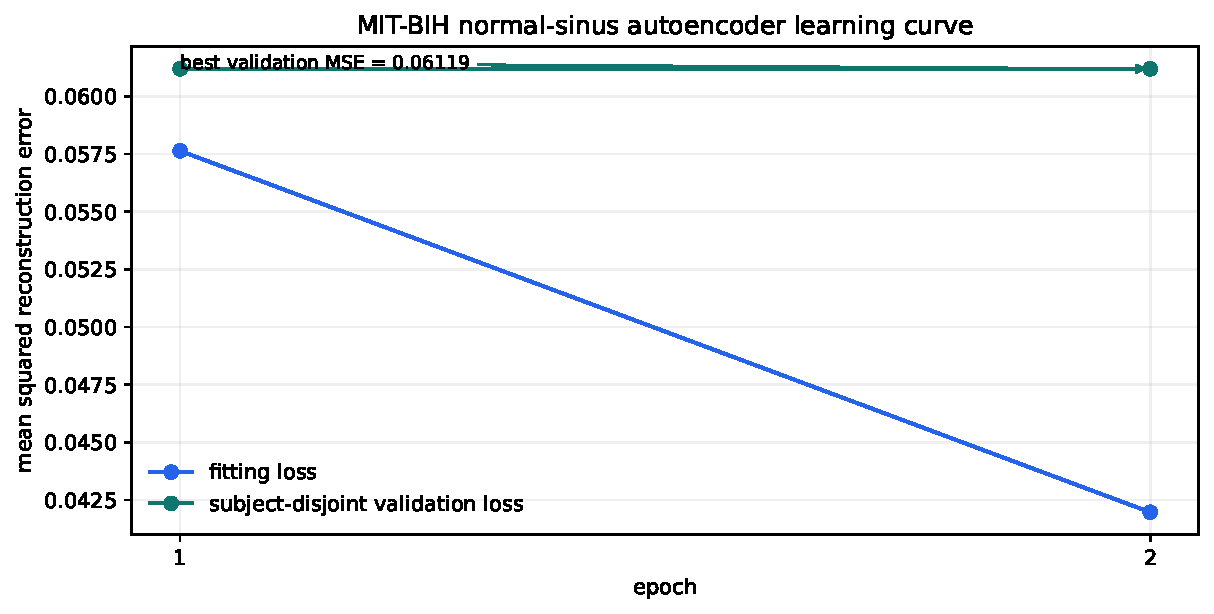
\includegraphics[width=.82\textwidth]{pic/generated/nsrdb_autoencoder_learning_curve.pdf}
\caption[Autoencoder fitting and validation loss.]{Autoencoder fitting and
subject-disjoint validation loss. The checkpoint with the lowest validation
loss is retained before the supervised MLII stages are trained.}
\label{fig:lead-ii-ae-learning}
\end{figure}

\subsection{Four autoencoder residual features}

Let $e_t=x_t-\widehat x_t$ be the reconstruction residual. The final feature
system uses four scalar residual summaries:
\begin{align}
 f_1&=\frac{1}{512}\sum_t|e_t| &&\text{whole-window MAE},\\
 f_2&=\frac{1}{512}\sum_te_t^2 &&\text{whole-window MSE},\\
 f_3&=\frac{1}{240}\sum_{t=104}^{343}|e_t| &&\text{central morphology MAE},\\
 f_4&=\frac{1}{511}\sum_{t=2}^{512}|e_t-e_{t-1}| &&\text{residual-change MAE}.
\end{align}
The central feature focuses on the QRS and nearby morphology. The
residual-change feature becomes large when the reconstruction misses sharp
slopes. These four values are appended to the transparent MLII and RR features.

\begin{figure}[H]
\centering
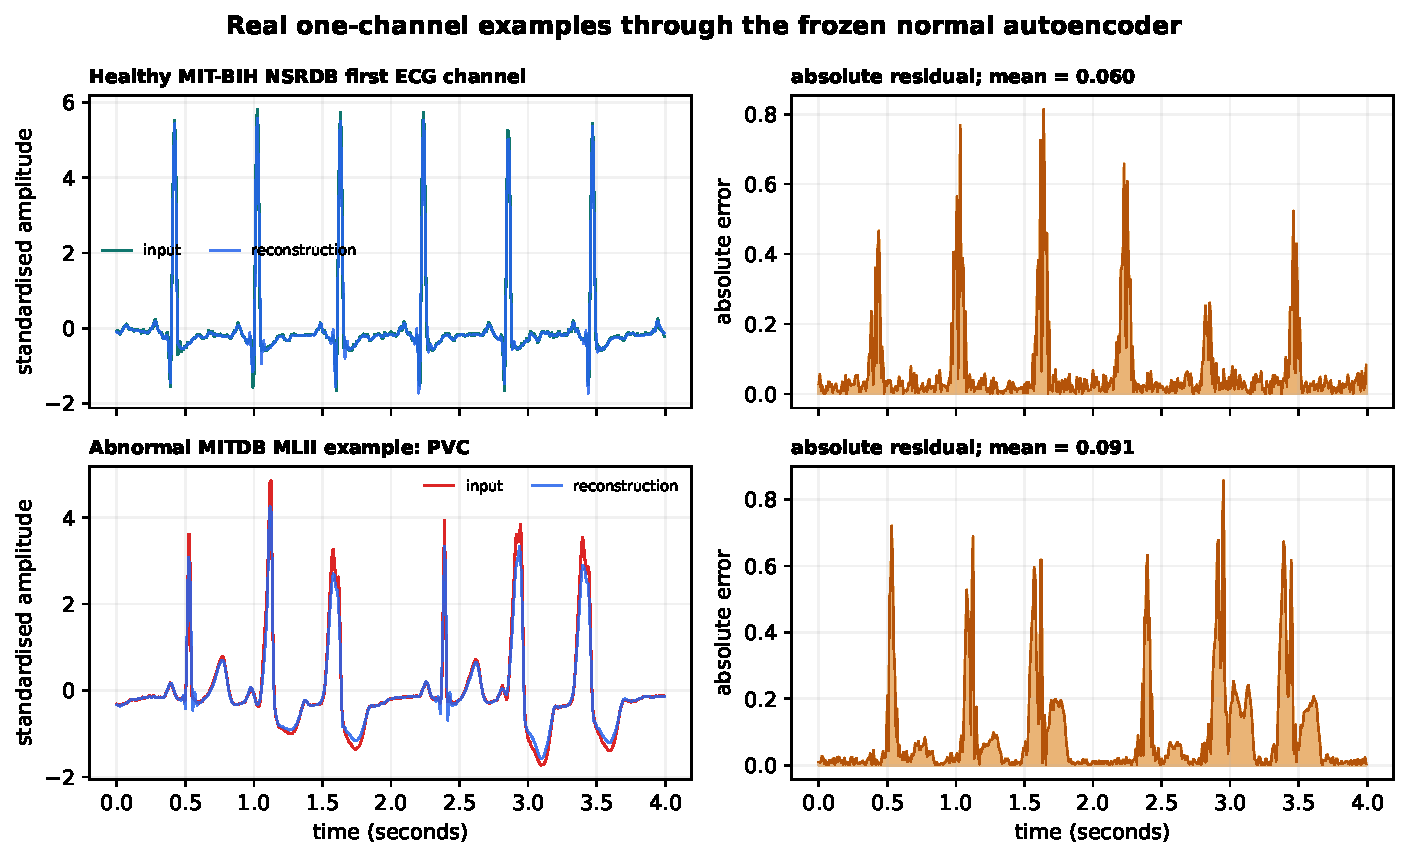
\includegraphics[width=.96\textwidth]{pic/generated/real_autoencoder_processing.pdf}
\caption{Real healthy and abnormal ECG examples through the frozen
autoencoder. The residual between input and reconstruction is converted into
four numerical features for the supervised detector.}
\label{fig:final-real-ae}
\end{figure}

\section{Final 242-value feature vector}

The saved final bundle declares 242 total features, 15 RR features, required
autoencoder features, and four autoencoder residual values. Therefore every
supervised prediction uses:
\begin{equation}
\begin{aligned}
&223\ \text{waveform/spectrum/statistics values}\\
&\quad +15\ \text{RR timing values}\\
&\quad +4\ \text{autoencoder residual values}=242.
\end{aligned}
\end{equation}

\begin{figure}[H]
\centering
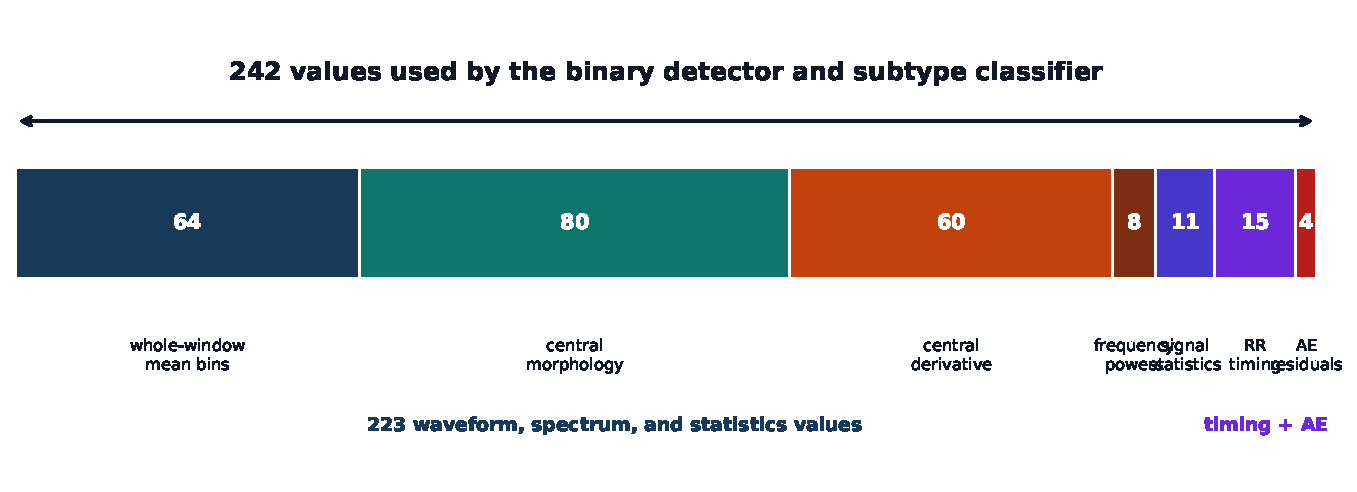
\includegraphics[width=.98\textwidth]{pic/generated/architecture_feature_vector.pdf}
\caption{Feature-vector layout used by both supervised models. The same
242-value vector is passed first to the abnormality detector and, if required,
to the subtype classifier.}
\label{fig:architecture-feature-vector}
\end{figure}

\begin{table}[H]
\centering
\caption{Organised feature groups in the final architecture.}
\label{tab:final-feature-vector}
\begin{tabular}{lrp{8.2cm}}
\toprule
Group & Values & What it tells the model\\
\midrule
Whole-window mean bins & 64 & broad four-second MLII waveform shape\\
Central morphology bins & 80 & P--QRS--T shape around the R peak\\
Central derivative bins & 60 & sharp slopes and rapid QRS changes\\
Frequency-band powers & 8 & relative energy from 0.5 to 50 Hz\\
Signal statistics & 11 & scale, range, energy, skewness, and kurtosis\\
RR timing context & 15 & previous/next interval, local rate, variability,
median, interquartile range, MAD, RMSSD, pNN50, range ratio, trend, and latest
RR change\\
Autoencoder residuals & 4 & how strongly the beat disagrees with the learned
normal-reconstruction pattern\\
\bottomrule
\end{tabular}
\end{table}

The final experiment constructs the same 242 values in two steps: first 230
values are built from 223 MLII waveform/statistical values plus seven base RR
values; then eight causal RR-history values and four autoencoder residual
values are appended. During live/session prediction, the backend builds the
same final vector directly from 223 MLII waveform/statistical values, 15 RR
values, and four autoencoder residual values.

\section{Binary abnormality detector}

The first supervised model is the abnormality detector. It receives all 242
features and estimates $p_i=P(\mathrm{abnormal}\mid x_i)$ for beat $i$. The
selected detector is an Extra Trees classifier with:
\begin{itemize}
\item 240 trees;
\item entropy split criterion;
\item fully grown trees;
\item minimum leaf size of one sample;
\item square-root feature sampling at each split;
\item record/class weighting with record-power $\alpha=0.35$.
\end{itemize}
The decision threshold was selected on the 64--80\% validation region of each
development record:
\begin{equation}
 a_i=\mathbb{1}[p_i>0.5708333].
\end{equation}
If $a_i=0$, the final output is normal class N. No subtype classifier is used
for that beat.

For tree $b$, let $p_b(x_i)$ be the abnormal class proportion in the reached
leaf. The ensemble probability is
\begin{equation}
 p_i=\frac{1}{240}\sum_{b=1}^{240}p_b(x_i).
\end{equation}
Averaging many randomly split trees reduces the instability of one decision
tree while still modelling non-linear links among ECG shape, RR timing, and
autoencoder residuals.

\section{Abnormal-subtype classifier}

The second supervised model is used only after the binary gate marks a beat as
abnormal. It is fitted only on supported abnormal classes 1--5, not on N and
not on unsupported MIT--BIH symbols. The selected subtype model is an Extra
Trees classifier with:
\begin{itemize}
\item 260 trees;
\item entropy split criterion;
\item fully grown trees;
\item minimum leaf size of one sample;
\item one-third feature sampling at each split;
\item record/class weighting with record-power $\alpha=0.25$.
\end{itemize}

For an abnormal beat, the subtype classifier returns probabilities over the
five supported abnormal outputs: PVC, PAC, LBBB, RBBB, and AFib. The final
subtype is
\begin{equation}
 \widehat y_i=\arg\max_{c\in\{1,\ldots,5\}}q_{ic}.
 \label{eq:final-decision}
\end{equation}
The final saved bundle sets \texttt{reject\_low\_confidence=False}. Therefore
the evaluated and installed final pipeline do not add a post-hoc
``Unclassified abnormal'' rejection step; every gated abnormal beat receives
the subtype with the largest subtype probability.

The displayed subtype confidence is conditional on the abnormal branch. It
is an ensemble score, not a calibrated probability of disease. Unsupported
abnormalities can receive an incorrect supported subtype.

\section{Final decision logic}

The complete prediction rule is:
\begin{enumerate}
\item Validate that the input is a 512-sample MLII beat window and that 15 RR
features are available.
\item Reconstruct the same window with the frozen autoencoder.
\item Build the 242-value vector from MLII shape, RR timing, and four
autoencoder residual summaries.
\item Estimate $p_i=P(\mathrm{abnormal}\mid x_i)$ using the 240-tree binary
detector.
\item If $p_i\leq0.5708333$, output N with confidence $1-p_i$.
\item If $p_i>0.5708333$, run the 260-tree subtype model and output the
highest-probability supported subtype.
\end{enumerate}

This is the same hierarchy used in the final temporal-holdout evaluation. The
model does not use test labels while predicting. The labels are used only after
prediction to compute accuracy, F1, confusion matrices, and subject-clustered
uncertainty.

\section{Why this architecture was selected}

\begin{table}[H]
\centering
\caption{Reason for each major final-architecture decision.}
\label{tab:final-design-rationale}
\begin{tabular}{>{\raggedright\arraybackslash}p{3.6cm}>{\raggedright\arraybackslash}p{9.6cm}}
\toprule
Decision & Reason\\
\midrule
MLII-only supervised input & matches the signal available in 46 eligible
MIT--BIH records and avoids hidden two-lead assumptions\\
R-peak alignment & puts comparable cardiac events in comparable positions
inside every 512-sample window\\
Waveform and derivative bins & preserve beat morphology, including sharp QRS
changes\\
Frequency powers and statistics & add compact information about signal energy,
scale, and distribution\\
Fifteen RR features & represent local rate, premature beats, rhythm
irregularity, and recent interval trend using information reproducible during
streaming\\
Normal-only autoencoder & supplies a learned measure of disagreement with
normal ECG structure without requiring arrhythmia labels\\
Two-stage hierarchy & allows unsupported abnormal beats to count in binary
testing without forcing them into one of the five supported subtype labels\\
Extra Trees models & handle mixed feature scales and non-linear interactions
with reproducible tabular-model training\\
Temporal split with gap & evaluates later signal from each record while
removing direct boundary overlap between development and test beats\\
\bottomrule
\end{tabular}
\end{table}

The architecture is therefore best described as a known-patient temporal
continuation system. Its final performance numbers describe later MLII signal
from patients whose earlier MLII signal was available during model development.
They should not be presented as unseen-patient generalisation without a
separate patient-disjoint evaluation.
